\chapter[Nuclear Reactions in Stars]{\textbf{Nuclear Reactions \\ in Stars}}
\label{chap:reactions}

\section{Introduction}

% I might not need an introduction section, but keep for now.

%%%%%%%%%%%%%%%%%%%%%%%%%%%%%%%%%%%%%%%%%%%%%%%%%%%%%%%%%%%%%%%%%%%%%%%%%%%%%%%%%%%%%%%%%%%%%

\section{Reaction Rates} \label{sec:rates}

The reaction rate per particle pair in a stellar medium is given by
\begin{equation} \label{eqn:reaction_rate}
\left\langle \sigma v \right\rangle_{01} = \sqrt{\frac{8}{\pi \mu_{01}}} \, \frac{1}{(kT)^{3/2}} \int_{0}^{\infty} E \, \sigma(E) \, e^{-E/kT} \, dE,
\end{equation}
where $\mu_{01}$ is the reduced mass of particle 0 and particle 1, $\mu = M_{0}M_{1}/(M_{0}+M_{1})$; $k$ is the Boltzmann constant; $T$ is the stellar temperature; $E$ is the center-of-mass energy between the particles; and $\sigma(E)$ is the reaction cross section evaluated at $E$. The energy dependence of the cross section determines whether numerical integration must be performed. The formalism for reaction rate calculations therefore depends on whether $\sigma(E)$ is smoothly varying over energy or if it can be described by isolated resonances. In either scenario, the cross section can be separated into a Coulomb factor and a factor resulting only from nuclear structure. That is, the cross section can be rewritten as
\begin{equation} \label{eqn:S-factor}
\sigma(E) = \frac{1}{E} \, e^{-2 \pi \eta} \, S(E),
\end{equation}
where $S(E)$ is the astrophysical S-factor, governed by nuclear effects alone, and $\eta$ is the Sommerfeld parameter defined by $2 \pi \eta = \sqrt{2 \mu / E} \,  Z_{0} Z_{1} e^{2} / \hbar$, where $Z_{0}$ and $Z_{1}$ are the atomic numbers of the nuclei. The $1/E$ factor is included to cancel with the $E$ factor in the reaction rate. Substituting Eqn. \ref{eqn:S-factor} into Eqn. \ref{eqn:reaction_rate}, we have
\begin{equation} \label{eqn:reaction_rate_S-factor}
\left\langle \sigma v \right\rangle_{01} = \sqrt{\frac{8}{\pi \mu_{01}}} \, \frac{1}{(kT)^{3/2}} \int_{0}^{\infty} e^{-2 \pi \eta} \, e^{-E/kT} \, S(E) \, dE.
\end{equation}

The integrand in Eqn. \ref{eqn:reaction_rate_S-factor} is composed of the Gamow factor $e^{-2 \pi \eta}$, the Boltzmann factor $e^{-E/kT}$, and the astrophysical S-factor $S(E)$. The former two factors have a combined energy dependence of $e^{-\sqrt{1/E}} \, e^{-E}$, while the $S(E)$ energy dependence is based on the nuclear structure of the specific reaction. The overlap between the Gamow and Boltzmann factors is called the \emph{Gamow peak}, $e^{-2 \pi \eta} \, e^{-E/kT}$. This peak determines the energies at which the reaction will proceed in the stellar environment at the given temperature\footnote{This is a slight oversimplification, since there is a circumstance where this is not the case. For resonant reactions at high stellar temperatures, the resonances that contribute significantly to the reaction rate may occur below the Gamow peak \cite{Iliadis2015}.}. It has a maximum at
\begin{align}
E_{0} &= \left[ \left(\frac{\pi}{\hbar}\right)^{2} (Z_{0} Z_{1} e^{2})^{2} \left(\frac{m_{01}}{2}\right) (kT)^{2} \right]^{1/3} \nonumber \\
&= 0.1220 \left(Z_{0}^{2} Z_{1}^{2} \mu_{01} T_{9}^{2} \right)^{1/3} \,\, [\mathrm{MeV}]
\end{align}
where $T_{9}$ is the temperature in units of GK. The energy $E_{0}$ is the most probable energy for nonresonant reactions, where $S(E)$ varies smoothly. For resonant reactions, where $S(E)$ is described by a sharp Lorentzian function, the Gamow peak can still be a useful indicator of which resonances contribute significantly to the total reaction rate, particularly at lower resonance energies ($E_{r}^{\mathrm{c.m.}} \lesssim 0.5$ MeV). The Gamow peak can be approximated by a Gaussian function with a mean of $E_{0}$ and a $1/e$ width of
\begin{equation}
\Delta = \frac{4}{\sqrt{3}} \sqrt{E_{0} k T} = 0.2368 \left(Z_{0}^{2} Z_{1}^{2} \mu_{01} T_{9}^{5}\right)^{1/6} \,\, [\mathrm{MeV}].
\end{equation}
Thermonuclear reactions therefore mainly occur in the energy window from $E_{0} - \Delta/2$ to $E_{0} + \Delta/2$, known as the \emph{Gamow window}.

For the $^{39}\mathrm{K}(p,\gamma)^{40}\mathrm{Ca}$ reaction, discussed in Chapter \ref{ch:GC}, the Gamow window at temperatures of 100 MK occurs between about 140 keV and 230 keV, centered on about 185 keV. This situation is depicted in Figure \ref{fig:Gamow_Window}. The Gamow and Maxwell-Boltzmann factors are shown in red and green, respectively, while the combined Gamow peak is shown in blue. The Gamow window centered on $E_{0}$ is shown between the vertical dotted lines. As will be clear in Section \ref{subsec:resonance_contributions}, the $^{39}\mathrm{K}(p,\gamma)^{40}\mathrm{Ca}$ reaction rate is dominated by isolated resonances in the temperature range of astrophysical interest, occuring between about 90 keV to 450 keV.

\begin{figure}[t]
\begin{tikzpicture}
\node at (0,0) {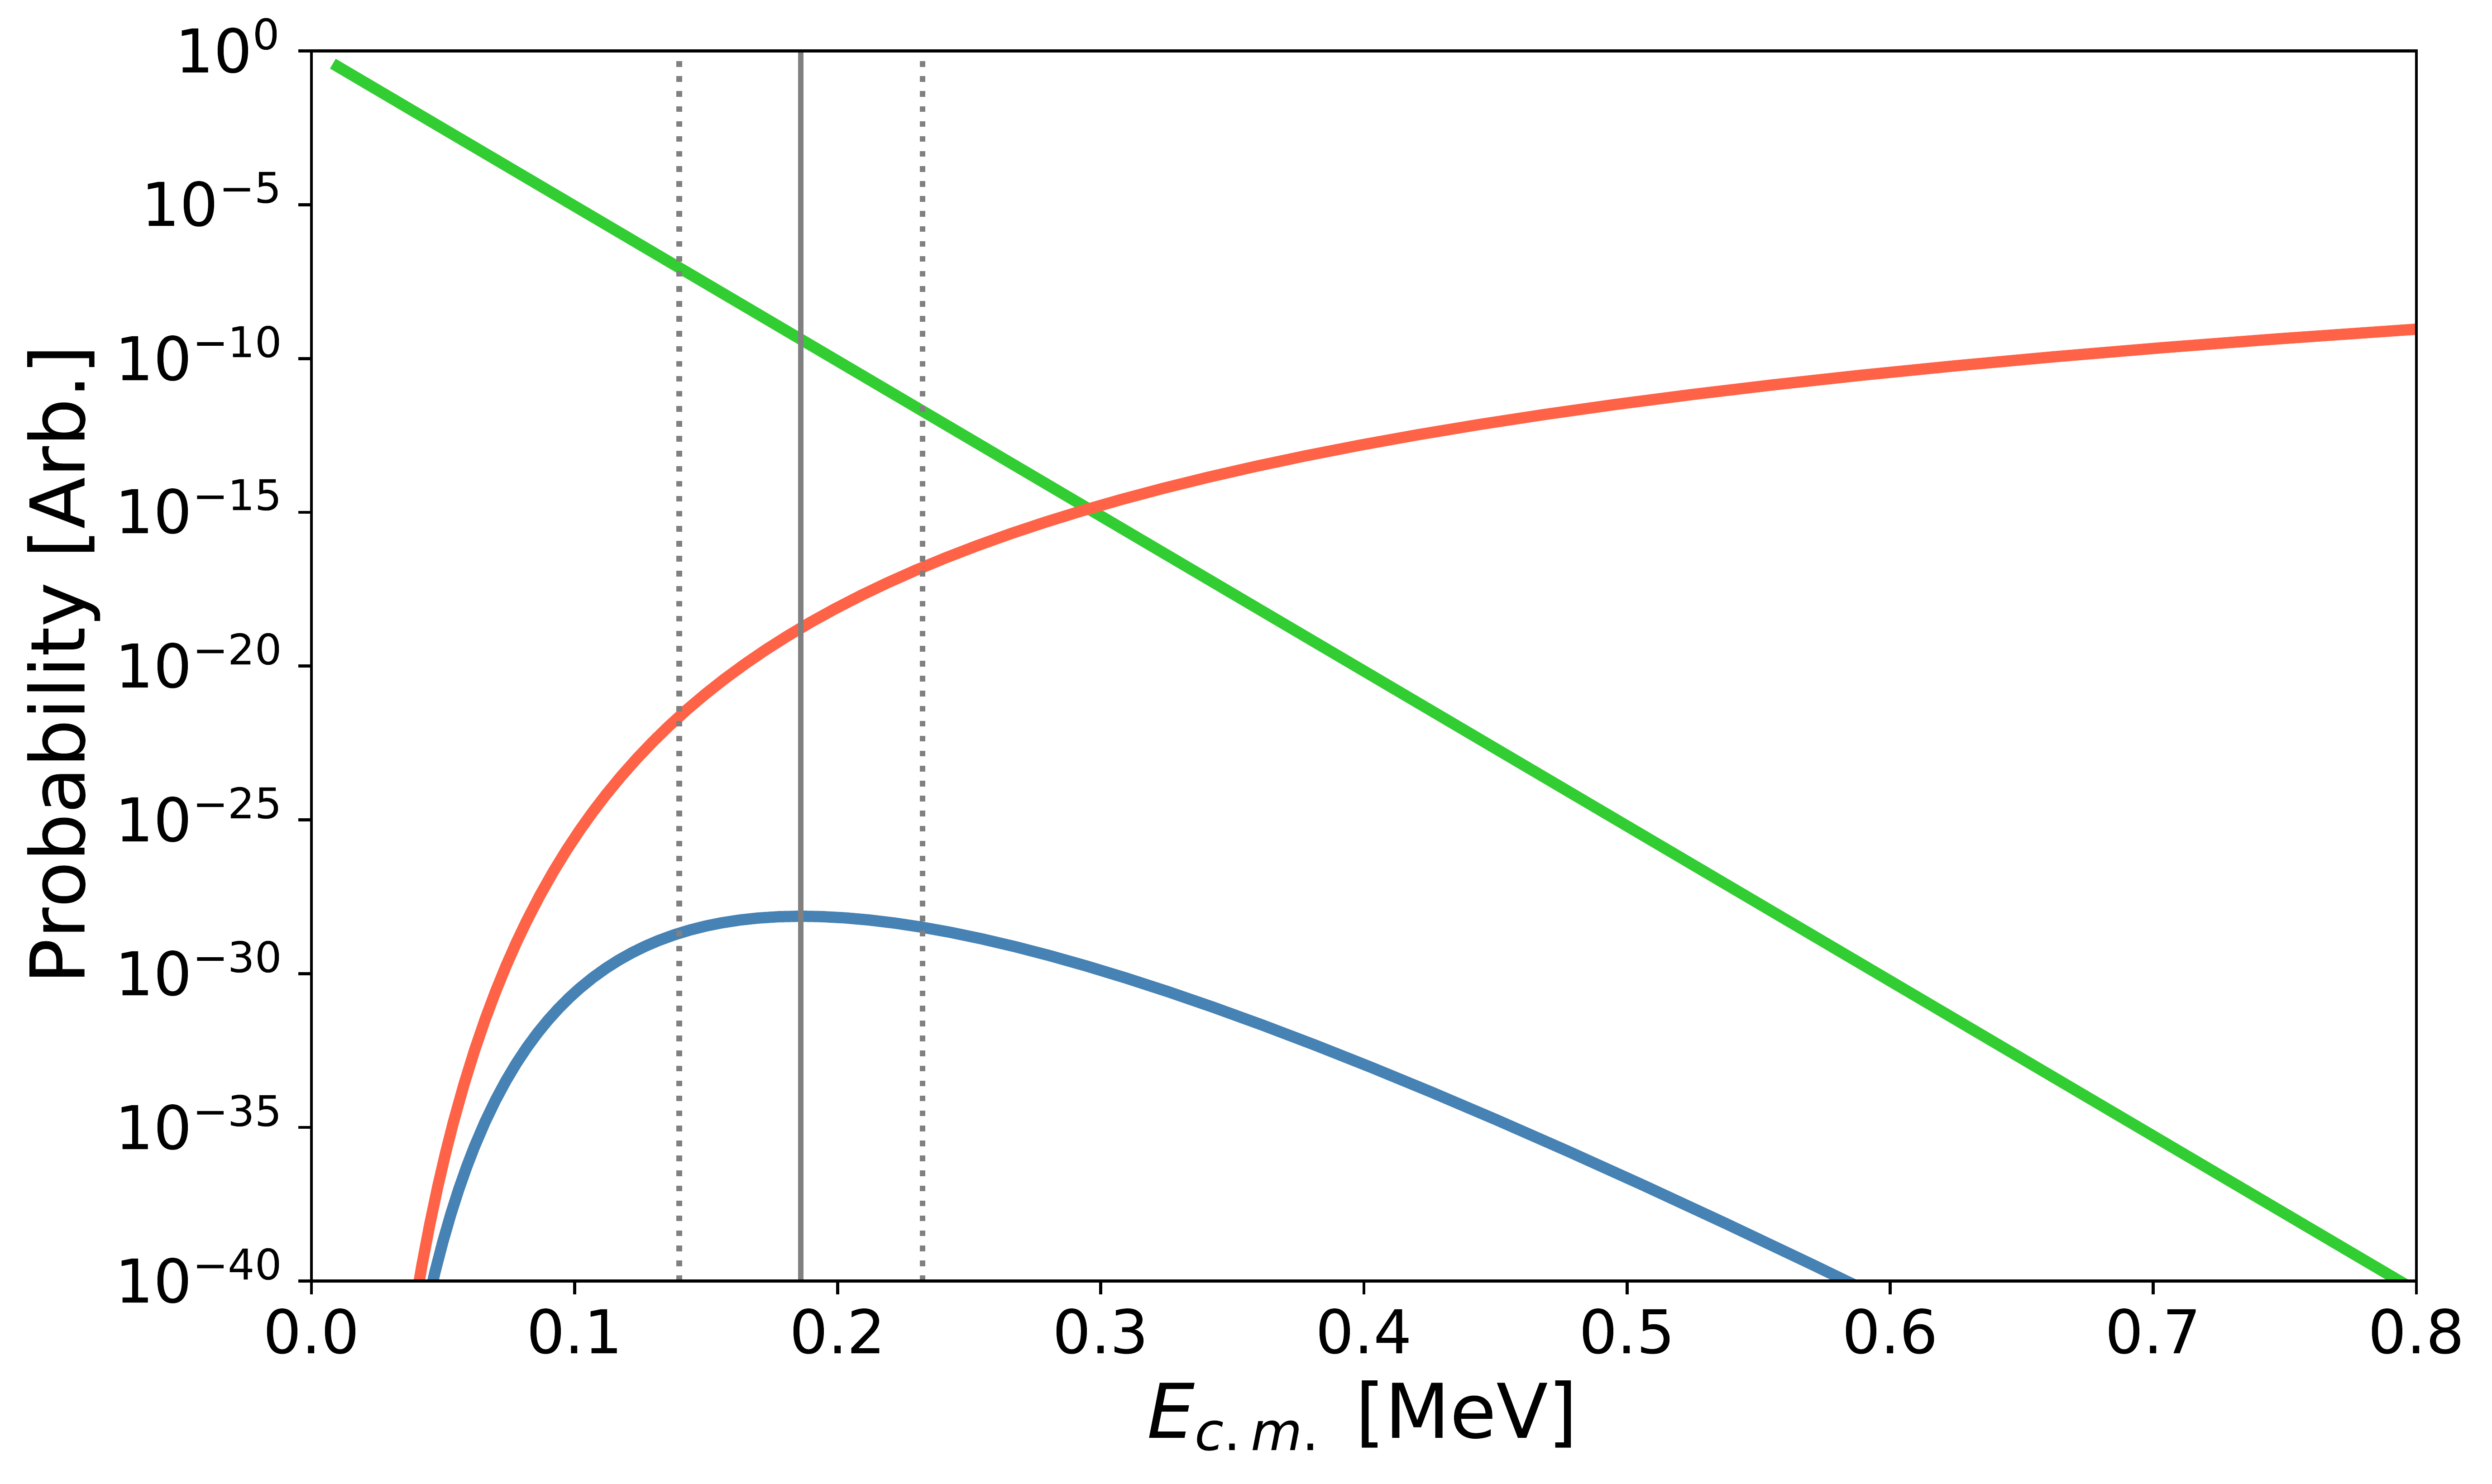
\includegraphics[width=6.5in]{Chapter-6/figs/Gamow_Window.png}};
\node at (5,3.15) {\Huge{$e^{-2\pi\eta}$}};
\node at (5,-0.5) {\Huge{$e^{-E/kT}$}};
\node[rotate=-20] at (1,-1.575) {\Huge{$e^{-2\pi\eta} e^{-E/kT}$}};
\node at (-5,2) {\large{$E_{0} \pm \frac{\Delta}{2}$}};
\draw[line width = 0.1 mm] (-4.9,1) -- (-3,1);
\draw[>=triangle 45, line width = 0.1 mm, ->] (-4.9,1) -- (-4.9,1.7);
\node at (0.5,3.9) (A) {\large{$T = 100$ MK}};
\node[draw=black, fit=(A)] {};
\end{tikzpicture}
\caption{\label{fig:Gamow_Window}The Gamow window, $E_{0} \pm \Delta/2$, for the $^{39}\mathrm{K}(p,\gamma)^{40}\mathrm{Ca}$ reaction at 100 MK. The Gamow factor $e^{-2 \pi \eta}$ is shown in red; the Maxwell-Boltzmann factor $e^{-E/kT}$ is shown in green; the Gamow peak $e^{-2 \pi \eta} e^{-E/kT}$ is shown in blue. The resonances that contribute significantly to the reaction rate at this temperature will have energies within the Gamow window.}
\end{figure}

\subsection{Narrow Resonances} \label{subsec:narrow_resonances}

% wg = wG_aG_b/G_tot <--- Resonance strength
% G_c = 2 P_c(E_r) g_c^{2} <--- Partial width
% g_c^{2} = (hbar^{2} / 2 \mu R) * C^{2}S \phi_{R}^{2} <--- single-particle reduced width
% R = R_{0}(A_{a}^{1/3} + A_{b}^{1/3}) <--- Channel radius
% \phi_{R}^{2} --> single-particle radial wave function at R
% C^{2}S <--- Spectroscopic factor

%%%%%%%%%%%%%%%%%%%%%%%%%%%%%%%%%%%%%%%%%%%%%%%%%%%%%%%%%%%%%%%%%%%%%%%%%%%%%%%%%%%%%%%%%%%%%

\section{Abundance Evolution}

% Equation from Christian's book that adds the production reactions and subtracts the destruction reactions, involving the reaction rates

%%%%%%%%%%%%%%%%%%%%%%%%%%%%%%%%%%%%%%%%%%%%%%%%%%%%%%%%%%%%%%%%%%%%%%%%%%%%%%%%%%%%%%%%%%%%%
\section{Transfer Reactions}

% This will be the last section of this chapter
% Theory leading to C2S and proton partial-width calculations

% Random Ch 6 note when I was going to discuss transfer reactions there:
%Chapter \ref{chap:reactions} described the proton-capture reaction rate as a function of experimental quantities, such as the proton partial-width $\Gamma_{p}$ and the $\gamma$-ray partial width $\Gamma_{\gamma}$. This section will describe how the proton partial-width

\subsection{Optical Model} \label{subsec:Optical_Model}

\subsection{Distorted Wave Born Approximation} \label{subsec:DWBA}

% Theoretical model, similar to Caleb's Section in his Chapter 2

% For a surface level explanation (good for defense questions! and for intro to section), see Krane pg. 421-424.

% Include Zero-range approximation

%\subsection{Spectroscopic Factors} \label{subsec:C2S}
% Might not need this section (should be covered in both Narrow Resonance and DWBA sections)
%\subsection{Proton Partial Widths} \label{subsec:PartialWidths}
% Might not need this section (should be covered in Narrow Resonance section)